\chapter{Условие}%
\label{cha:uslovie}

\section{Задача 1}%
\label{sec:task_1}
Назначить адреса подсетей:

\begin{enumerate}
    \item Подсеть 1: 192.168.x.0 /24
    \item Подсеть 2: 192.168.x+1.0 /24
    \item Подсеть 3: 192.168.x+2.0 /24
    \item Подсеть 4: 192.168.x+3.0 /24
    \item Подсеть 5 (В задаче III): 192.168.x+10.0 /24
\end{enumerate}

\section{Задача 2}%
\label{sec:task_2}

Настроить динамическую маршрутизацию в прилагаемом .pkt файле на стенде I через протокол RIPv2 так, чтобы пинг любым хостом или маршрутизатором любого другого хоста или маршрутизатора был успешным.

Представить отдельным .pkt файлом.
\section{Задание 3}
\label{sec:task_3}

Настроить динамическую маршрутизацию в сети в прилагаемом .pkt файле на стенде II через протокол OSPF так, чтобы пинг любым хостом или маршрутизатором любого другого хоста или маршрутизатора был успешным. Разделить при этом сеть на области OSPF в соответствии со схемой. Выполнить указания в лабораторной работе.

Представить отдельным .pkt файлом.

\chapter{Практическая часть}%
\label{cha:prakticheskaia_chast_}

\section{Задача 1}%
\label{sec:1}

Стенды были разделены на подсети, указанные в pkt файле. Изображения стендов представлены на рисунках ниже. 

\begin{figure}[H]
    \centering
    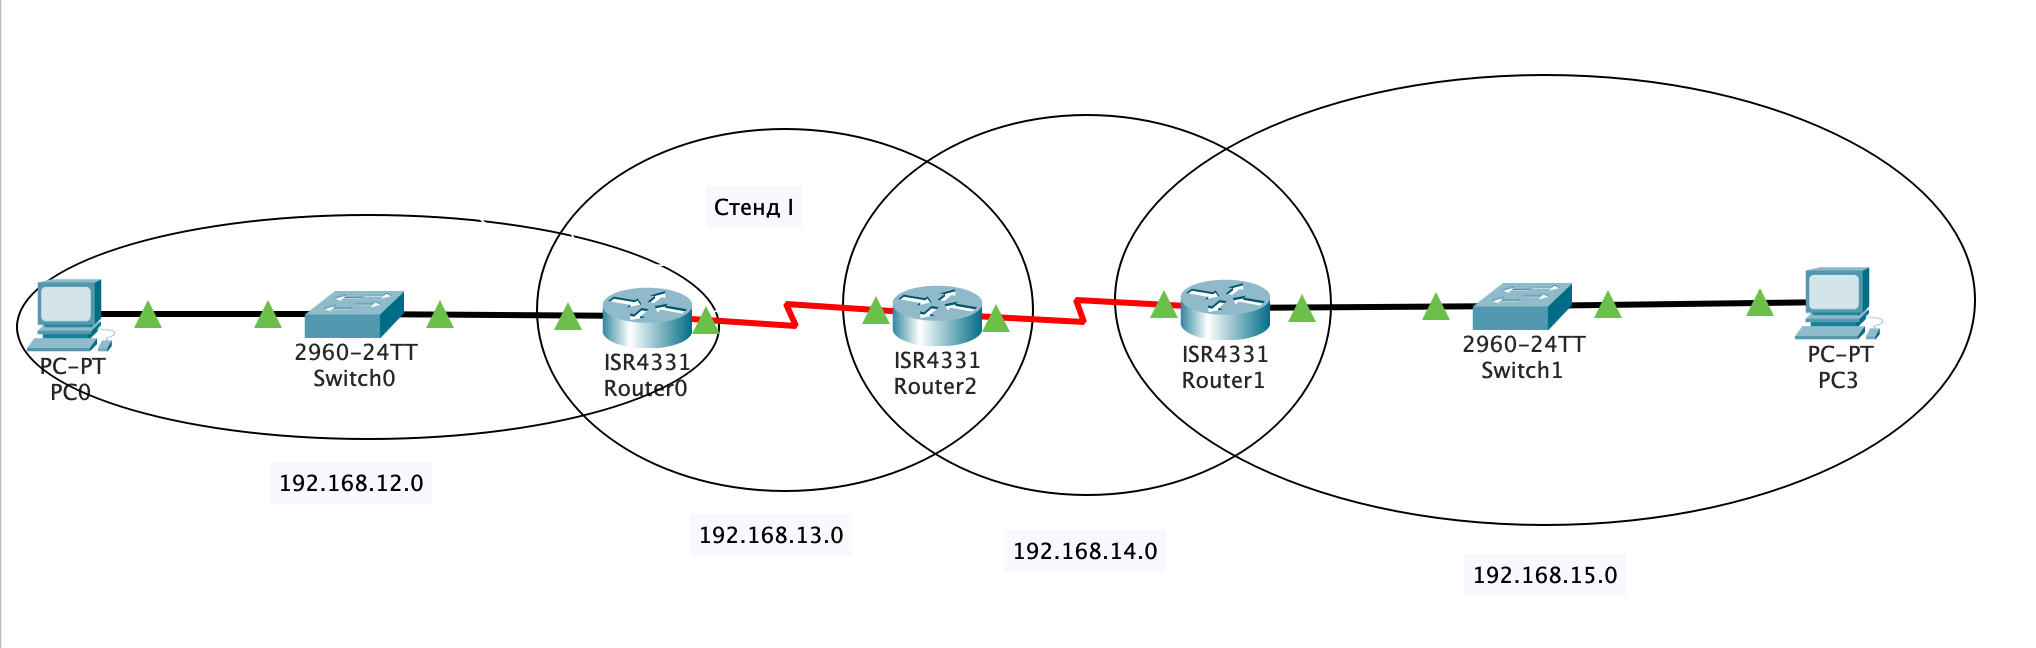
\includegraphics[width=1\textwidth]{images/1.png}
    \caption{Разделение на подсети на первом стенде}
    \label{fig:stand1}
\end{figure}

\begin{figure}[H]
    \centering
    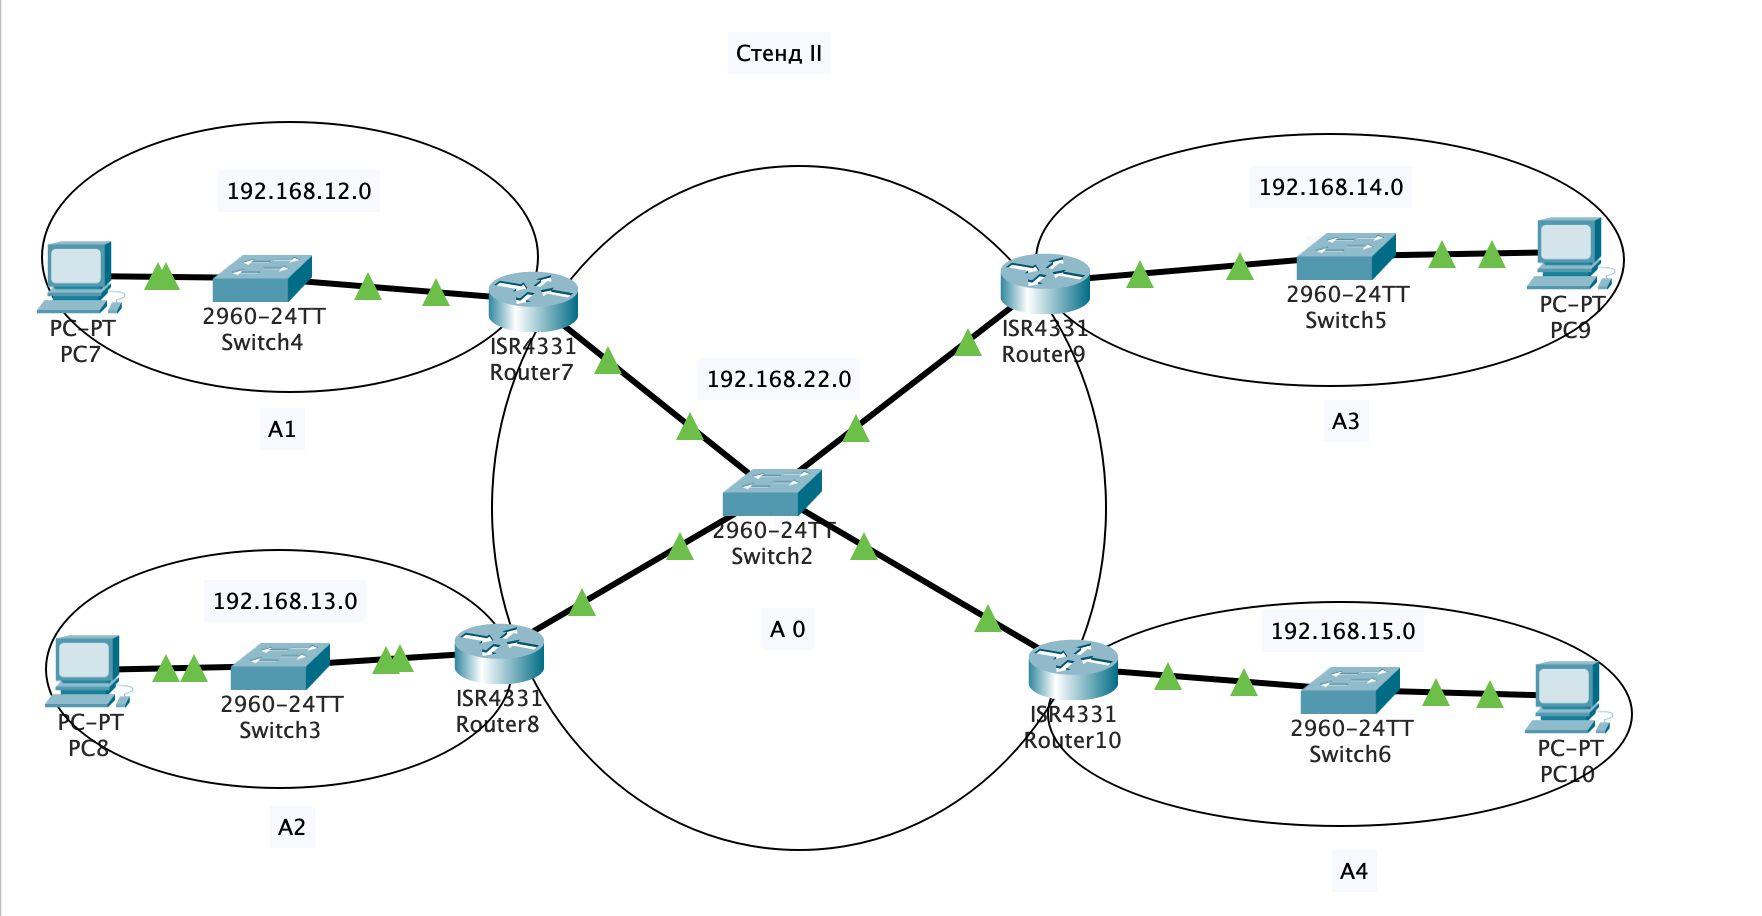
\includegraphics[width=1\textwidth]{images/stend_2.png}
    \caption{Разделение на подсети на втором стенде}
    \label{fig:stand2}
\end{figure}

\section{Задача 2}%
\label{sec:2}

Команды для настройки RIP на Router0 преведены на рисунке ниже. Для остальных роутеров команды аналогичны.

\begin{figure}[H]
    \centering
    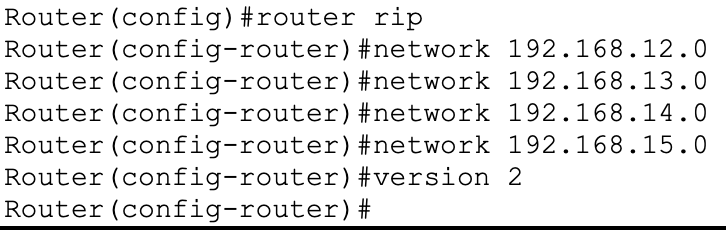
\includegraphics[width=0.8\textwidth]{images/2.png}
    \caption{Настройка RIP для Router0 с первого стенда}
    \label{fig:rip}
\end{figure}

На рисунке ниже представлен результат проверки соединения между PC0 и PC3 с помощью команды ping.

\begin{figure}[H]
    \centering
    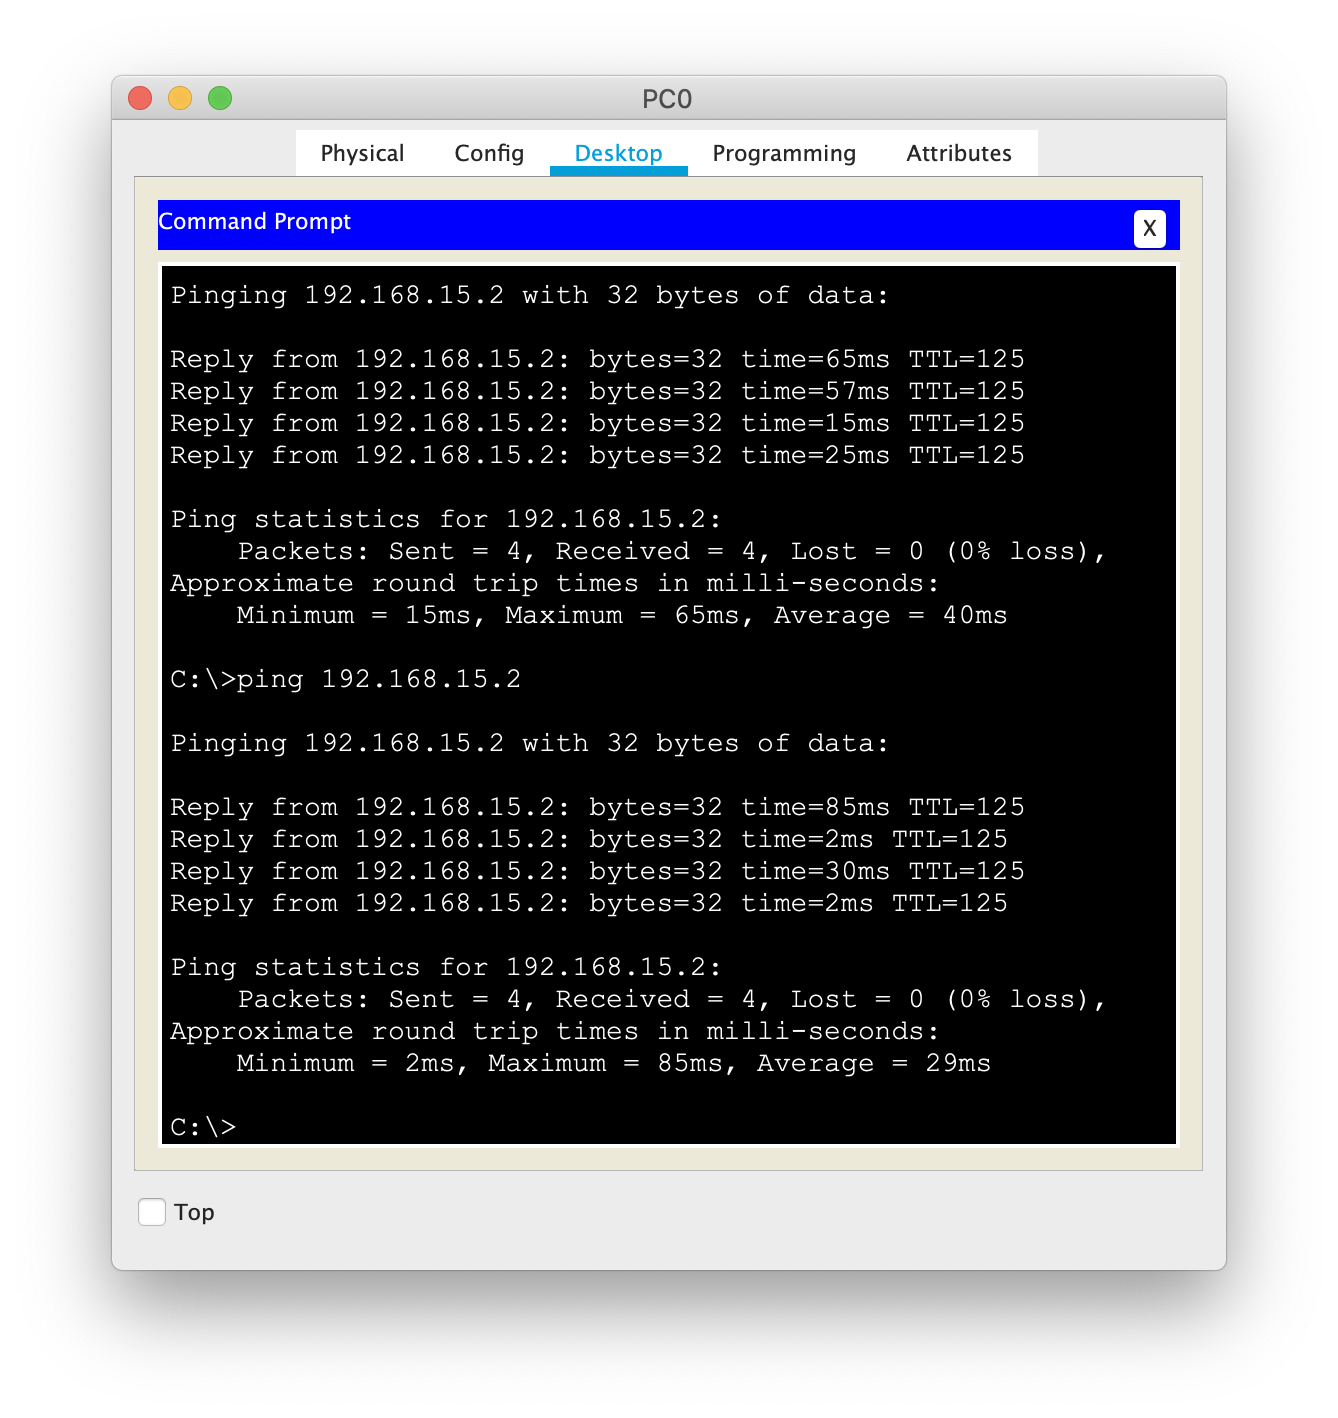
\includegraphics[width=0.8\textwidth]{images/ping_1.png}
    \caption{Проверка соединения между PC0 и PC3 с первого стенда}
    \label{fig:ping_1}
\end{figure}

\section{Задача 3}%
\label{sec:3}

Для работы протокола OSPF были настроены все роутеры. На рисунках ниже представлены команды для настройки каждого роутера.

\begin{figure}[H]
    \centering
    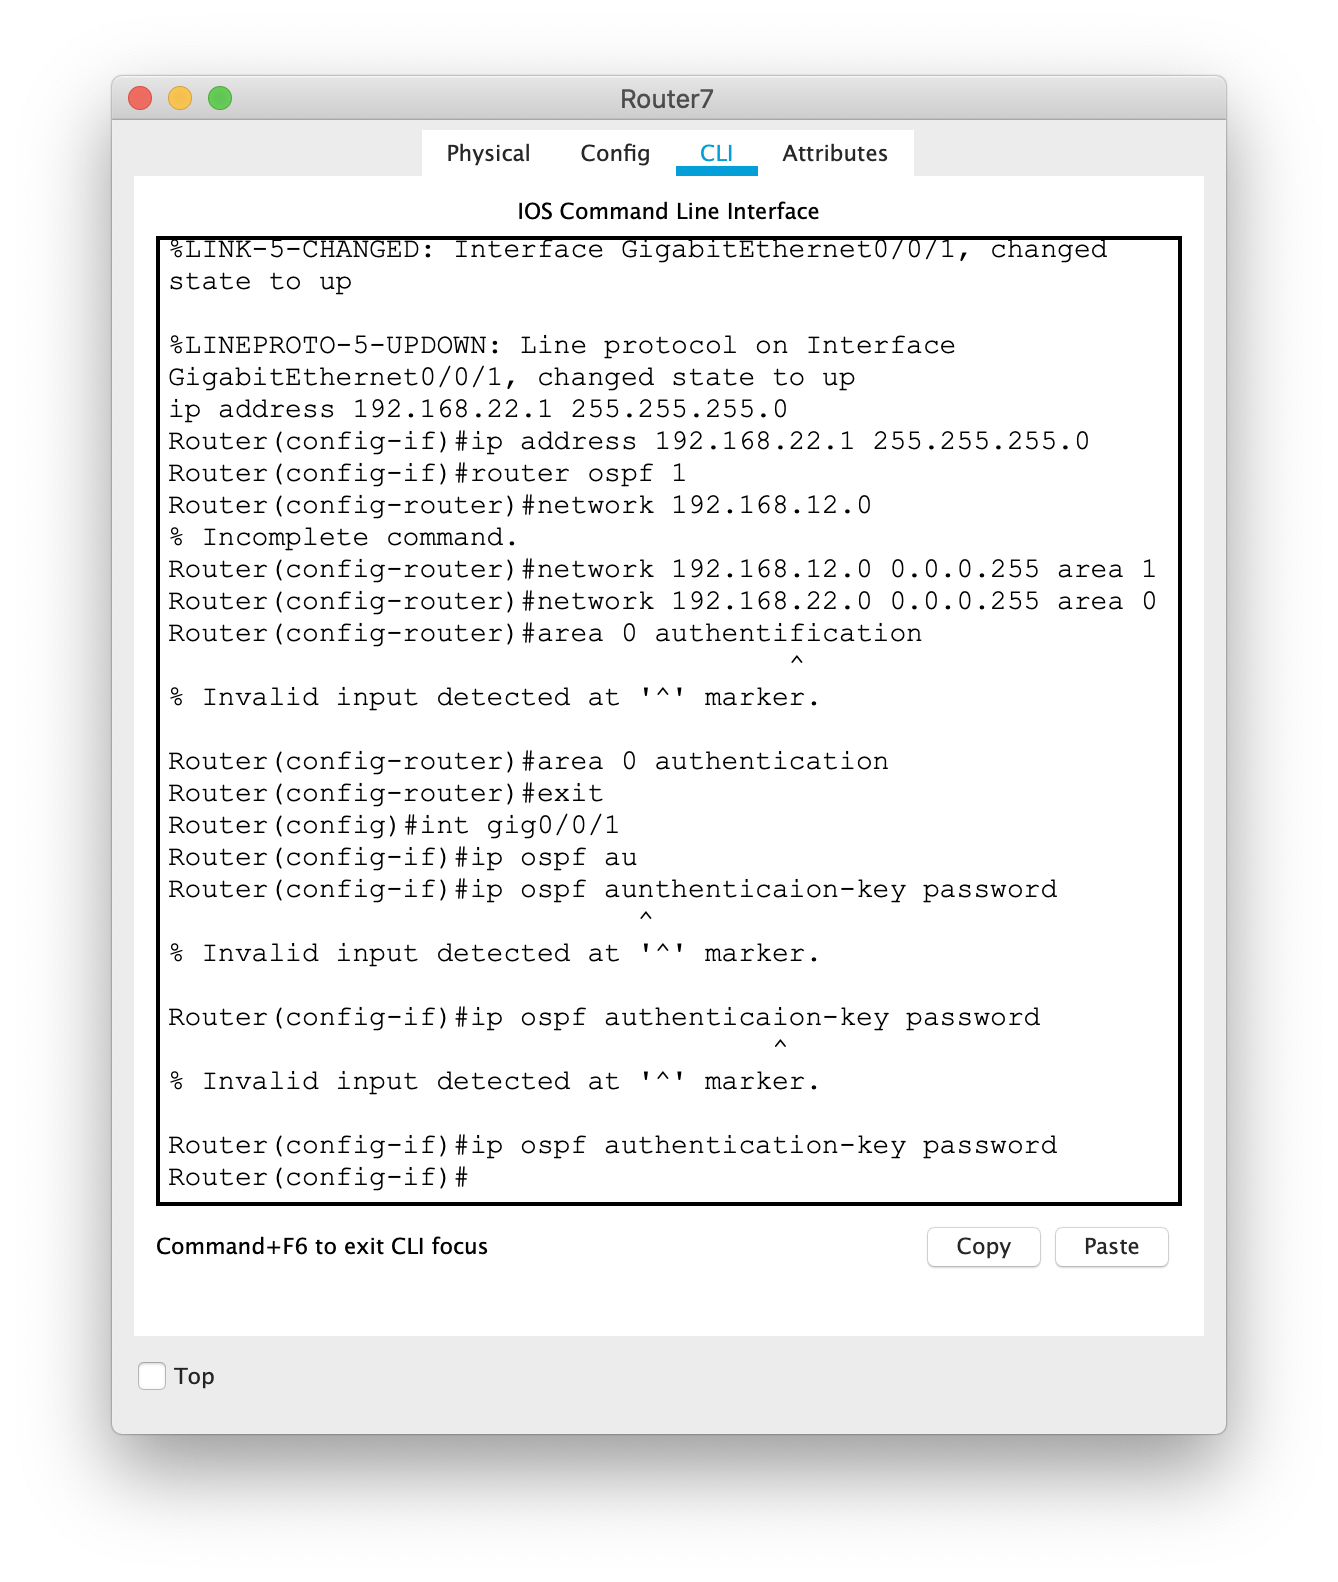
\includegraphics[width=0.8\textwidth]{images/pozor.png}
    \caption{Настройка OSPF для Router7}
    \label{fig:router7}
\end{figure}

\begin{figure}[H]
    \centering
    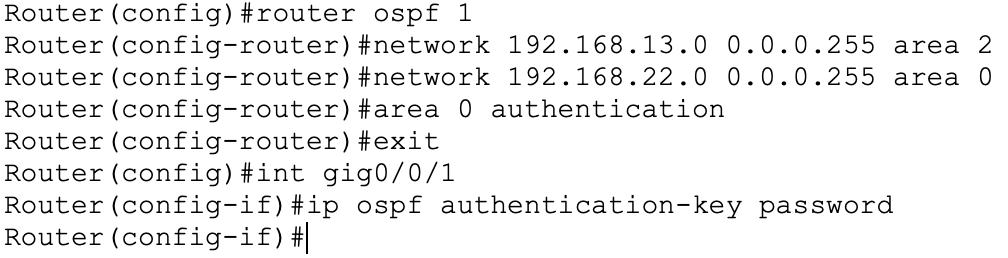
\includegraphics[width=0.8\textwidth]{images/pozor_2.png}
    \caption{Настройка OSPF для Router8}
    \label{fig:router8}
\end{figure}

\begin{figure}[H]
    \centering
    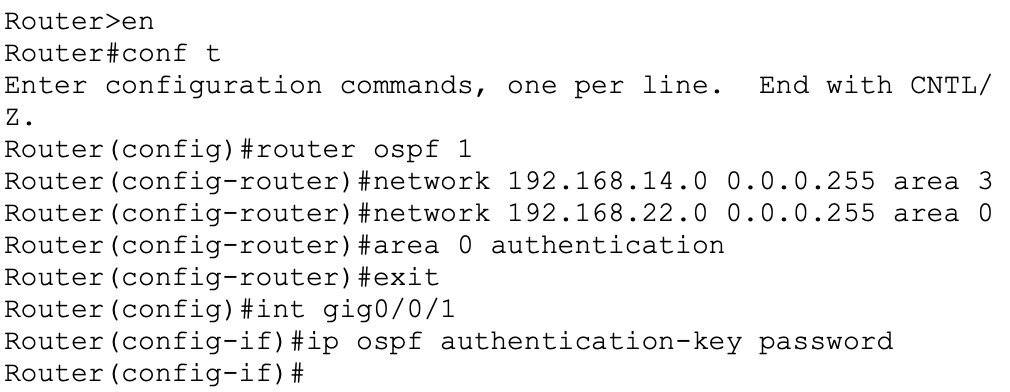
\includegraphics[width=0.8\textwidth]{images/pozor_3.png}
    \caption{Настройка OSPF для Router9}
    \label{fig:router9}
\end{figure}

\begin{figure}[H]
    \centering
    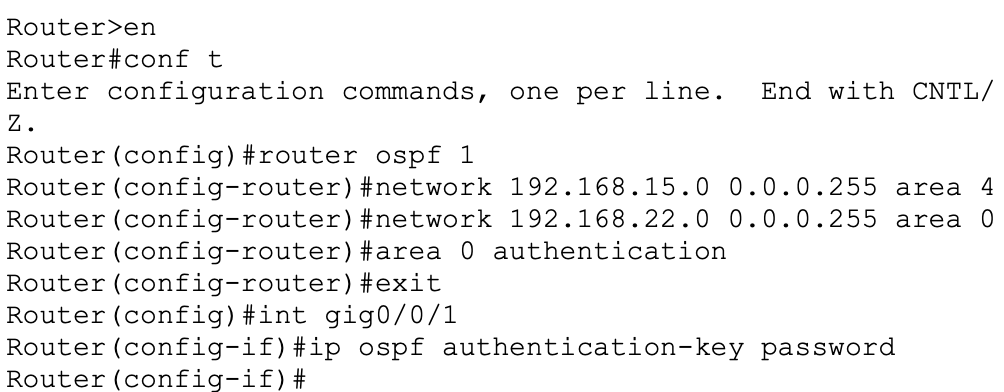
\includegraphics[width=0.8\textwidth]{images/pozor_4.png}
    \caption{Настройка OSPF для Router10}
    \label{fig:router10}
\end{figure}

Результат проверки статуса соседних устройств представлен на риснунке ниже:

\begin{figure}[H]
    \centering
    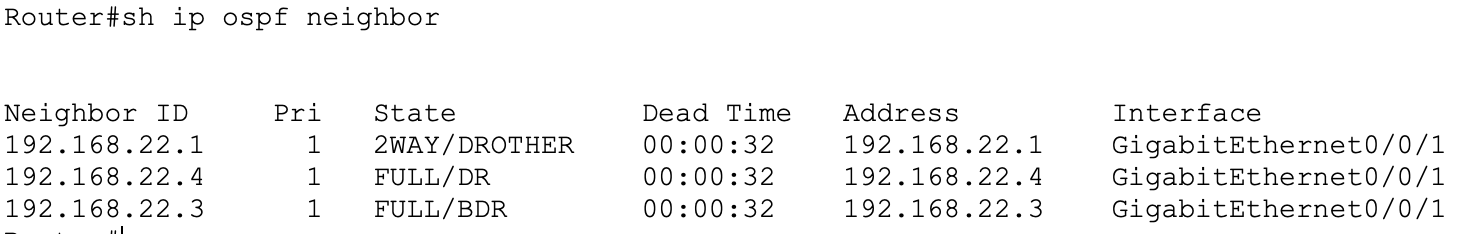
\includegraphics[width=0.8\textwidth]{images/prefinal.png}
    \caption{Информация о соседних устройствах для Router8}
    \label{fig:neighbor}
\end{figure}

Результат проверки соединения между PC7 и PC10 представлен на рисунке ниже.

\begin{figure}[H]
    \centering
    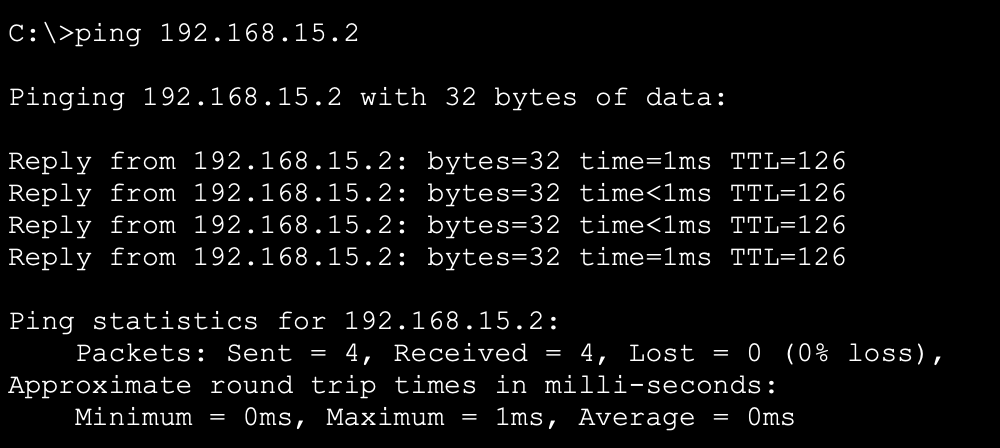
\includegraphics[width=0.8\textwidth]{images/final.png}
    \caption{Результат проверки соединения между PC7 и PC10}
    \label{fig:ping_2}
\end{figure}
